\documentclass{article}
%\documentstyle[11pt,handout,psfig]{article}

\usepackage{fullpage,amssymb,amsmath,epsf}
\usepackage[12pt]{extsizes}

%These give really tight margins:
%\setlength{\topmargin}{-0.3in}
%\setlength{\textheight}{8.10in}
%\setlength{\textwidth}{5.8in}
%\setlength{\baselineskip}{0.1875in}
%\addtolength{\leftmargin}{-2.775in}
%\setlength{\footskip}{0.45in}
%\setlength{\oddsidemargin}{0.5in}
%\setlength{\evensidemargin}{0.5in}
%%\setlength{\headsep}{0pt}
%%\setlength{\headheight}{0pt}

%\setlength{\topmargin}{-0.5in}
\setlength{\textheight}{8in}
%\setlength{\textwidth}{5.0in}
%\setlength{\baselineskip}{0.1875in}
%\addtolength{\leftmargin}{-2.775in}
%\setlength{\footskip}{0.45in}
%\setlength{\oddsidemargin}{0.5in}
%\setlength{\evensidemargin}{0.5in}
%%\setlength{\headsep}{0pt}
%%\setlength{\headheight}{0pt}


\newcommand{\Sbar}{\bar{S}}
\newcommand{\sbar}{\bar{s}}

%\markright{CS229 Winter 2003}
\pagestyle{myheadings}

\newcommand{\newsec}{\section}
\newcommand{\denselist}{\itemsep 0pt\partopsep 0pt}
\newcommand{\bitem}{\begin{itemize}\denselist}
\newcommand{\eitem}{\end{itemize}}
\newcommand{\benum}{\begin{enumerate}\denselist}
\newcommand{\eenum}{\end{enumerate}}

\newcommand{\fig}[1]{\private{\begin{center}
{\Large\bf ({#1})}
\end{center}}}

\newcommand{\cpsf}[1]{{\centerline{\psfig{#1}}}}
\newcommand{\mytitle}[1]{\centerline{\LARGE\bf #1}}

\newcommand{\myw}{{\bf w}}

\newcommand{\mypar}[1]{\vspace{1ex}\noindent{\bf {#1}}}

\def\thmcolon{\hspace{-.85em} {\bf :} }

\newtheorem{THEOREM}{Theorem}[section]
\newenvironment{theorem}{\begin{THEOREM} \thmcolon }%
                        {\end{THEOREM}}
\newtheorem{LEMMA}[THEOREM]{Lemma}
\newenvironment{lemma}{\begin{LEMMA} \thmcolon }%
                      {\end{LEMMA}}
\newtheorem{COROLLARY}[THEOREM]{Corollary}
\newenvironment{corollary}{\begin{COROLLARY} \thmcolon }%
                          {\end{COROLLARY}}
\newtheorem{PROPOSITION}[THEOREM]{Proposition}
\newenvironment{proposition}{\begin{PROPOSITION} \thmcolon }%
                            {\end{PROPOSITION}}
\newtheorem{DEFINITION}[THEOREM]{Definition}
\newenvironment{definition}{\begin{DEFINITION} \thmcolon \rm}%
                            {\end{DEFINITION}}
\newtheorem{CLAIM}[THEOREM]{Claim}
\newenvironment{claim}{\begin{CLAIM} \thmcolon \rm}%
                            {\end{CLAIM}}
\newtheorem{EXAMPLE}[THEOREM]{Example}
\newenvironment{example}{\begin{EXAMPLE} \thmcolon \rm}%
                            {\end{EXAMPLE}}
\newtheorem{REMARK}[THEOREM]{Remark}
\newenvironment{remark}{\begin{REMARK} \thmcolon \rm}%
                            {\end{REMARK}}
%\newenvironment{proof}{\noindent {\bf Proof:} \hspace{.677em}}%
%                      {}

%theorem
\newcommand{\thm}{\begin{theorem}}
%lemma
\newcommand{\lem}{\begin{lemma}}
%proposition
\newcommand{\pro}{\begin{proposition}}
%definition
\newcommand{\dfn}{\begin{definition}}
%remark
\newcommand{\rem}{\begin{remark}}
%example
\newcommand{\xam}{\begin{example}}
%corollary
\newcommand{\cor}{\begin{corollary}}
%proof
\newcommand{\prf}{\noindent{\bf Proof:} }
%end theorem
\newcommand{\ethm}{\end{theorem}}
%end lemma
\newcommand{\elem}{\end{lemma}}
%end proposition
\newcommand{\epro}{\end{proposition}}
%end definition
\newcommand{\edfn}{\bbox\end{definition}}
%end remark
\newcommand{\erem}{\bbox\end{remark}}
%end example
\newcommand{\exam}{\bbox\end{example}}
%end corollary
\newcommand{\ecor}{\end{corollary}}
%end proof
\newcommand{\eprf}{\bbox\vspace{0.1in}}
%begin equation
\newcommand{\beqn}{\begin{equation}}
%end equation
\newcommand{\eeqn}{\end{equation}}

%\newcommand{\eqref}[1]{Eq.~\ref{#1}}

\newcommand{\KB}{\mbox{\it KB\/}}
\newcommand{\infers}{\vdash}
\newcommand{\sat}{\models}
\newcommand{\bbox}{\vrule height7pt width4pt depth1pt}

\newcommand{\act}[1]{\stackrel{{#1}}{\rightarrow}}
\newcommand{\at}[1]{^{(#1)}}

\newcommand{\argmax}{{\rm argmax}}

\newcommand{\rimp}{\Rightarrow}
\newcommand{\dimp}{\Leftrightarrow}

\newcommand{\bX}{\mbox{\boldmath $X$}}
\newcommand{\bY}{\mbox{\boldmath $Y$}}
\newcommand{\bZ}{\mbox{\boldmath $Z$}}
\newcommand{\bU}{\mbox{\boldmath $U$}}
\newcommand{\bE}{\mbox{\boldmath $E$}}
\newcommand{\bx}{\mbox{\boldmath $x$}}
\newcommand{\be}{\mbox{\boldmath $e$}}
\newcommand{\by}{\mbox{\boldmath $y$}}
\newcommand{\bz}{\mbox{\boldmath $z$}}
\newcommand{\bu}{\mbox{\boldmath $u$}}
\newcommand{\bd}{\mbox{\boldmath $d$}}
\newcommand{\smbx}{\mbox{\boldmath $\scriptstyle x$}}
\newcommand{\smbd}{\mbox{\boldmath $\scriptstyle d$}}
\newcommand{\smby}{\mbox{\boldmath $\scriptstyle y$}}
\newcommand{\smbe}{\mbox{\boldmath $\scriptstyle e$}}


\newcommand{\word}[1]{\mbox{\it #1\/}}
\newcommand{\Action}{\word{Action}}
\newcommand{\Proposition}{\word{Proposition}}
\newcommand{\true}{\word{true}}
\newcommand{\false}{\word{false}}
\newcommand{\Pre}{\word{Pre}}
\newcommand{\Add}{\word{Add}}
\newcommand{\Del}{\word{Del}}
\newcommand{\Result}{\word{Result}}
\newcommand{\Regress}{\word{Regress}}
\newcommand{\Maintain}{\word{Maintain}}

\newcommand{\bor}{\bigvee}
\newcommand{\invert}[1]{{#1}^{-1}}

\newcommand{\commentout}[1]{}

\newcommand{\bmu}{\mbox{\boldmath $\mu$}}
\newcommand{\btheta}{\mbox{\boldmath $\theta$}}
\newcommand{\IR}{\mbox{$I\!\!R$}}

\newcommand{\tval}[1]{{#1}^{1}}
\newcommand{\fval}[1]{{#1}^{0}}

\newcommand{\tr}{{\rm tr}}
\newcommand{\vecy}{{\vec{y}}}
\renewcommand{\Re}{{\mathbb R}}

\def\twofigbox#1#2{%
\noindent\begin{minipage}{\textwidth}%
\epsfxsize=0.35\maxfigwidth
\noindent \epsffile{#1}\hfill
\epsfxsize=0.35\maxfigwidth
\epsffile{#2}\\
\makebox[0.35\textwidth]{(a)}\hfill\makebox[0.35\textwidth]{(b)}%
\end{minipage}}

\def\twofigboxcd#1#2{%
\noindent\begin{minipage}{\textwidth}%
\epsfxsize=0.35\maxfigwidth
\noindent \epsffile{#1}\hfill
\epsfxsize=0.35\maxfigwidth
\epsffile{#2}\\
\makebox[0.35\textwidth]{(c)}\hfill\makebox[0.35\textwidth]{(d)}%
\end{minipage}}

\def\twofigboxnolabel#1#2{%
\begin{minipage}{\textwidth}%
\epsfxsize=0.35\maxfigwidth
\noindent \epsffile{#1}\hfill
\epsfxsize=0.35\maxfigwidth
\epsffile{#2}\\
%\makebox[0.48\textwidth]{(a)}\hfill\makebox[0.48\textwidth]{(b)}%
\end{minipage}
}

\def\twofigboxnolabelFive#1#2{%
\begin{minipage}{\textwidth}%
\hbox to 0.5in{}\epsfxsize=0.35\maxfigwidth
\noindent \epsffile{#1}\hfill
\epsfxsize=0.35\maxfigwidth
\epsffile{#2}\hbox to 0.5in{}\\
%\makebox[0.48\textwidth]{(a)}\hfill\makebox[0.48\textwidth]{(b)}%
\end{minipage}
}

\def\threefigbox#1#2#3{%
\noindent\begin{minipage}{\textwidth}%
\epsfxsize=0.33\maxfigwidth
\noindent \epsffile{#1}\hfill
\epsfxsize=0.33\maxfigwidth
\noindent \epsffile{#2}\hfill 
\epsfxsize=0.33\maxfigwidth
\epsffile{#3}\\
\makebox[0.31\textwidth]{{\scriptsize (a)}}\hfill%
\makebox[0.31\textwidth]{{\scriptsize (b)}}\hfill
\makebox[0.31\textwidth]{{\scriptsize (c)}}%
\smallskip
\end{minipage}}

\def\threefigboxnolabel#1#2#3{%
\noindent\begin{minipage}{\textwidth}%
\epsfxsize=0.33\maxfigwidth
\noindent \epsffile{#1}\hfill
\epsfxsize=0.33\maxfigwidth
\noindent \epsffile{#2}\hfill 
\epsfxsize=0.33\maxfigwidth
\epsffile{#3}\\
%\makebox[0.31\textwidth]{{\scriptsize (a)}}\hfill%
%\makebox[0.31\textwidth]{{\scriptsize (b)}}\hfill
%\makebox[0.31\textwidth]{{\scriptsize (c)}}%
%\smallskip
\end{minipage}}

\newlength{\maxfigwidth}
\setlength{\maxfigwidth}{\textwidth}
%\def\captionsize {\footnotesize}
\def\captionsize {}

\newcommand{\xsi}{{x^{(i)}}}
\newcommand{\xsd}{{x^{(d)}}}
\newcommand{\xsj}{{x^{(j)}}}
\newcommand{\ysi}{{y^{(i)}}}
\newcommand{\ysj}{{y^{(j)}}}
\newcommand{\gsi}{{\gamma^{(i)}}}
\newcommand{\wsi}{{w^{(i)}}}
\newcommand{\esi}{{\epsilon^{(i)}}}

\newcommand{\calM}{{\cal M}}
\newcommand{\calH}{{\cal H}}
\newcommand{\calN}{{\cal N}}
\newcommand{\calX}{{\cal X}}
\newcommand{\calY}{{\cal Y}}
\newcommand{\calL}{{\cal L}}
\newcommand{\calP}{{\cal P}}
\newcommand{\calD}{{\cal D}}
\newcommand{\calF}{{\cal F}}

\newcommand{\ytil}{{\tilde{y}}}

\newcommand{\Ber}{{\rm Bernoulli}}
\newcommand{\MI}{{\rm MI}}
\newcommand{\E}{{\rm E}}

\newcommand{\pstar}{{p^{\ast}}}
\newcommand{\bstar}{{b^{\ast}}}
\newcommand{\dstar}{{d^{\ast}}}
\newcommand{\wstar}{{w^{\ast}}}
\newcommand{\alphastar}{\alpha^{\ast}}
\newcommand{\alphastari}{{\alpha_i^{\ast}}}
\newcommand{\betastar}{{\beta^{\ast}}}
\newcommand{\tol}{{\textit tol}}
\newcommand{\phihat}{\hat\phi}
\newcommand{\ehat}{\hat\varepsilon}
\newcommand{\hhat}{\hat{h}}
\newcommand{\hstar}{h^\ast}
\newcommand{\VC}{{\rm VC}}

\newcommand{\Strain}{S_{\rm train}}
\newcommand{\Scv}{{S_{\rm cv}}}

\newcommand{\hwb}{{h_{w,b}}}

\usepackage{graphicx}
\usepackage{subcaption}
%\renewcommand{\epsffile}[1]{
%	\includegraphics[width=\epsfxsize]{#1}
%}

\newcommand{\di}{{d}}
\newcommand{\nexp}{{n}}
\newcommand{\vcd}{{\textbf{D}}}

\begin{document}
\title{XCS229ii Lecture Notes}
\author{Andrew Ng}
\date{}
\maketitle


\setcounter{part}{12}
\part{Reinforcement Learning and Control}

We now begin our study of reinforcement learning and adaptive control.

In supervised learning, we saw algorithms that tried to make their outputs
mimic the labels $y$ given in the training set.  In that setting, the labels
gave an unambiguous
``right answer'' for each of the inputs $x$.  In contrast, for many sequential
decision making and control problems, it is very difficult to provide this
type of
explicit supervision to a learning algorithm.  For example, if we
have just built a four-legged robot and are trying to program it to walk, then
initially we have no idea what the ``correct'' actions to take are to make it
walk, and so do not
know how to provide explicit supervision for a learning algorithm to try to mimic.

In the reinforcement learning framework, we will instead provide our algorithms
only a reward function, which indicates to the learning agent when it
is doing well, and when it is doing poorly.
In the four-legged walking example, the reward function might give the
robot positive rewards for moving forwards, and negative rewards for
either moving backwards or falling over.  It will then be the learning
algorithm's job to figure out how to choose actions over time so as
to obtain large rewards.

Reinforcement learning has been successful in applications as diverse as
autonomous helicopter flight, robot legged locomotion, cell-phone network
routing, marketing strategy selection, factory control, and efficient
web-page indexing.
Our study of reinforcement learning will begin with a definition of the
{\bf Markov decision processes (MDP)}, which provides the formalism in which
RL problems are usually posed.

\section{Markov decision processes}

A Markov decision process is a tuple $(S,A, \{P_{sa}\}, \gamma, R)$, where:
\begin{itemize}
\item $S$ is a set of {\bf states}.  (For example, in autonomous helicopter flight,
$S$ might be the set of all possible positions and orientations of the helicopter.)
\item $A$ is a set of {\bf actions}. (For example, the set of all possible directions
in which you can push the helicopter's control sticks.)
\item $P_{sa}$ are the state transition probabilities.  For each state
$s\in S$ and action $a \in A$, $P_{sa}$ is a distribution over the state space.
We'll say more about this later, but briefly, $P_{sa}$ gives the
distribution over what states we will transition to if we take
action $a$ in state $s$.
\item $\gamma \in [0, 1)$ is called the {\bf discount factor}.
\item $R : S \times A \mapsto \Re$ is the {\bf reward function}.
(Rewards are sometimes also written as a function of a state $S$ only, in
which case we would have $R : S \mapsto \Re$).
\end{itemize}

The dynamics of an MDP proceeds as follows:
We start in some state $s_0$, and get to choose some action $a_0 \in A$ to take
in the MDP.  As a result of our choice, the state of the MDP
randomly transitions to some successor state $s_1$, drawn according
to $s_1 \sim P_{s_0a_0}$.  Then, we get to pick another action $a_1$.
As a result of this action, the state transitions again, now to
some $s_2 \sim P_{s_1a_1}$.  We then pick $a_2$, and so on\ldots.  Pictorially,
we can represent this process as follows:
\[
s_0 \stackrel{a_0}{\longrightarrow} s_1
\stackrel{a_1}{\longrightarrow} s_2
\stackrel{a_2}{\longrightarrow} s_3
\stackrel{a_3}{\longrightarrow} \ldots
\]

Upon visiting the sequence of states $s_0, s_1, \ldots$ with actions $a_0, a_1, \ldots$,
our total payoff is given by
\[
R(s_0, a_0) + \gamma R(s_1, a_1) + \gamma^2 R(s_2, a_2) + \cdots.
\]
Or, when we are writing rewards as a function of the states only, this becomes
\[
R(s_0) + \gamma R(s_1) + \gamma^2 R(s_2) + \cdots.
\]
For most of our development, we will use the simpler state-rewards $R(s)$, though
the generalization to state-action rewards $R(s,a)$ offers no special difficulties.

Our goal in reinforcement learning is to choose actions over time so as
to maximize the expected value of the total payoff:
\[
\E\left[R(s_0) + \gamma R(s_1) + \gamma^2 R(s_2) + \cdots\right]
\]
Note that the reward at timestep $t$ is {\bf discounted} by a factor of $\gamma^t$.
Thus, to make this expectation large, we would like to accrue positive rewards
as soon as possible (and postpone negative rewards as long as possible).  In
economic applications where $R(\cdot)$ is the amount of money made, $\gamma$ also has
a natural interpretation in terms of the interest rate (where a dollar today is
worth more than a dollar tomorrow).

A {\bf policy} is any function $\pi: S \mapsto A$ mapping from the states to the
actions.  We say that we are {\bf executing} some policy $\pi$ if, whenever we are
in state $s$, we take action $a = \pi(s)$.  We also define the {\bf value function}
for a policy $\pi$ according to
\[
V^\pi(s) =
\E\left[R(s_0) + \gamma R(s_1) + \gamma^2 R(s_2) + \cdots\right | s_0 = s, \pi].
\]
$V^\pi(s)$ is simply the expected sum of discounted rewards upon starting
in state $s$, and taking actions according to $\pi$.\footnote{This notation
in which we condition on $\pi$ isn't technically correct because $\pi$ isn't
a random variable, but this is quite standard in the literature.}

Given a fixed policy $\pi$, its value function $V^\pi$ satisfies the
{\bf Bellman equations}:
\[
V^\pi(s) = R(s) + \gamma \sum_{s' \in S} P_{s\pi(s)}(s')V^\pi(s').
\]
This says that the expected sum of discounted rewards $V^\pi(s)$ for
starting in $s$ consists of two terms: First, the {\bf immediate reward}
$R(s)$ that we get right away simply for starting in state $s$, and second,
the expected sum of future discounted rewards.  Examining the second term
in more detail, we see that the summation term above can be rewritten
$\E_{s' \sim P_{s\pi(s)}}[ V^\pi(s')]$.  This is the expected sum of
discounted rewards for starting in state $s'$, where $s'$ is distributed
according $P_{s\pi(s)}$, which is the distribution over where we will end
up after taking the first action $\pi(s)$ in the MDP from state $s$.
Thus, the second term above gives the expected sum of discounted rewards
obtained \emph{after} the first step in the MDP.

Bellman's equations can be used to efficiently solve for $V^\pi$.  Specifically,
in a finite-state MDP ($|S| < \infty$), we can write down one such equation
for $V^\pi(s)$ for every state $s$.  This gives us a set of $|S|$ linear
equations in $|S|$ variables (the unknown $V^\pi(s)$'s, one for each state), which
can be efficiently solved for the $V^\pi(s)$'s.

We also define the {\bf optimal value function} according to
\begin{equation}
\Vstar(s) = \max_{\pi} V^\pi(s).
\label{eqn-vstar}
\end{equation}
In other words, this is the best possible expected sum of discounted rewards
that can be attained using any policy.  There is also a version of Bellman's
equations for the optimal value function:
\begin{equation}
\Vstar(s) = R(s) + \max_{a \in A} \gamma \sum_{s'\in S} P_{sa}(s')\Vstar(s').
\label{eqn-optbellman}
\end{equation}
The first term above is the immediate reward as before.  The second term is
the maximum over all actions $a$ of the expected future sum of discounted
rewards we'll get upon after action $a$.  You should make sure you understand
this equation and see why it makes sense.

We also define a policy $\pistar : S \mapsto A$ as follows:
\begin{equation}
\pistar(s) = \arg \max_{a \in A} \sum_{s'\in S} P_{sa}(s')\Vstar(s').
\label{eqn-pistar}
\end{equation}
Note that $\pistar(s)$ gives the action $a$ that attains the maximum in
the ``max'' in Equation~(\ref{eqn-optbellman}).

It is a fact that for every state $s$ and every policy $\pi$, we have
\[
\Vstar(s) = V^{\pistar}(s) \geq V^\pi(s).
\]
The first equality says that the $V^{\pistar}$, the value function
for $\pistar$, is equal to the optimal value function $\Vstar$ for every state $s$.
Further, the inequality above says that $\pistar$'s value is at least a large
as the
value of any other other policy.  In other words, $\pistar$ as defined in
Equation~(\ref{eqn-pistar}) is the optimal policy.

Note that $\pistar$ has the interesting property that it is the
optimal policy for \emph{all} states $s$.  Specifically, it is not the case
that if we were starting in some state $s$ then there'd be some optimal policy
for that state, and if we were starting in some other state $s'$ then there'd
be some other policy that's optimal policy for $s'$.  The same
policy $\pistar$ attains the maximum in Equation~(\ref{eqn-vstar}) for
\emph{all} states $s$.  This means that we can
use the same policy $\pistar$ no matter what the
initial state of our MDP is.


\section{Value iteration and policy iteration} \label{sec-viandpi}

We now describe two efficient algorithms for solving finite-state MDPs.  For now,
we will consider only MDPs with finite state and action spaces ($|S| < \infty,\;
|A| < \infty$). In this section, we will also assume that we know the state transition probabilities $\{P_{sa}\}$ and the reward function $R$. 

The first algorithm, {\bf value iteration}, is as follows:
\begin{enumerate}
\item For each state $s$, initialize $V(s) := 0$.
\item Repeat until convergence $\{$
\begin{itemize}
\item[] For every state, update
$V(s) := R(s) + \max_{a \in A} \gamma \sum_{s'} P_{sa}(s') V(s')$.
\end{itemize}
\item[] $\}$
\end{enumerate}
This algorithm can be thought of as repeatedly trying to update the estimated
value function using Bellman Equations~(\ref{eqn-optbellman}).

There are two possible ways of performing the updates in the inner loop of the
algorithm.  In the first, we can first compute the new values for $V(s)$ for
every state $s$, and then overwrite all the old values with the new values.  This
is called a {\bf synchronous} update.  In this case, the algorithm can be
viewed as implementing a ``Bellman backup operator'' that takes a current estimate
of the value function, and maps it to a new estimate.  (See homework problem for
details.)  Alternatively, we can also perform {\bf asynchronous} updates.
Here, we would loop over the states (in some order), updating the values one at
a time.

Under either synchronous or asynchronous updates, it can be shown that
value iteration will cause $V$ to converge to $\Vstar$.
Having found $\Vstar$, we can then use Equation~(\ref{eqn-pistar}) to
find the optimal policy.

Apart from value iteration, there is a second standard algorithm for finding
an optimal policy for an MDP.  The {\bf policy iteration} algorithm proceeds as
follows:
\begin{enumerate}
\item Initialize $\pi$ randomly.
\item Repeat until convergence $\{$
\begin{enumerate}
\item Let $V := V^\pi$.
\item For each state $s$, let
$\pi(s) := \arg \max_{a \in A} \sum_{s'} P_{sa}(s') V(s')$.
\end{enumerate}
\item[] $\}$
\end{enumerate}
Thus, the inner-loop repeatedly computes the value function for the current
policy, and then updates the policy using the current value function.  (The policy
$\pi$ found in step (b) is also called the policy that is {\bf greedy with respect
to $V$}.) Note that step (a) can be done via solving Bellman's equations as
described earlier, which in the case of a fixed policy, is just a set
of $|S|$ linear equations in $|S|$ variables.

After at most a finite number of iterations of this algorithm,
$V$ will converge to $\Vstar$, and $\pi$ will converge to $\pistar$.

Both value iteration and policy iteration are standard algorithms for solving
MDPs, and there isn't currently universal agreement over which algorithm is better.
For small MDPs, policy iteration is often very
fast and converges with very few iterations.  However, for MDPs with large
state spaces, solving for $V^\pi$ explicitly would involve solving a large
system of linear equations, and could be difficult.  In these problems,
value iteration may be preferred.  For this reason, in practice
value iteration seems to be used more often than policy iteration.

\section{Learning a model for an MDP}

So far, we have discussed MDPs and algorithms for MDPs assuming that the
state transition probabilities and rewards are known.  In many realistic problems,
we are not given state transition probabilities and rewards explicitly, but
must instead estimate them from data.  (Usually, $S, A$ and $\gamma$ are known.)

For example, suppose that, for the inverted pendulum problem (see problem set 4),
we had a number of trials in the MDP, that proceeded as follows:
\begin{eqnarray*}
&s_0^{(1)} \stackrel{a_0^{(1)}}{\longrightarrow} s_1^{(1)}
\stackrel{a_1^{(1)}}{\longrightarrow} s_2^{(1)}
\stackrel{a_2^{(1)}}{\longrightarrow} s_3^{(1)}
\stackrel{a_3^{(1)}}{\longrightarrow} \ldots  \\
&s_0^{(2)} \stackrel{a_0^{(2)}}{\longrightarrow} s_1^{(2)}
\stackrel{a_1^{(2)}}{\longrightarrow} s_2^{(2)}
\stackrel{a_2^{(2)}}{\longrightarrow} s_3^{(2)}
\stackrel{a_3^{(2)}}{\longrightarrow} \ldots  \\
&\ldots  \hbox to 2.4in{}
\end{eqnarray*}

Here, $s_i^{(j)}$ is the state we were at time $i$ of trial $j$, and
$a_i^{(j)}$ is the corresponding action that was taken from that state.
In practice, each of the trials above might be run until the MDP terminates
(such as if the pole falls over in the inverted pendulum problem), or it might
be run for some large but finite number of timesteps.

Given this ``experience'' in the MDP consisting of a number of trials, we
can then easily derive the maximum likelihood estimates for the state
transition probabilities:
\begin{equation}
P_{sa}(s') = \frac{\hbox{\#times took we action $a$ in state $s$ and got to $s'$}}%
{\hbox{\#times we took action a in state $s$}}
\label{eqn-estpsa}
\end{equation}
Or, if the ratio above is ``0/0''---corresponding to the case of never having
taken action $a$ in state $s$ before---the we might simply estimate $P_{sa}(s')$ to
be $1/|S|$.  (I.e., estimate $P_{sa}$ to be the uniform distribution over all states.)

Note that, if we gain more experience (observe more trials) in the MDP, there is
an efficient way to update our estimated state transition probabilities using
the new experience.
Specifically, if we keep around the counts for both the numerator and
denominator terms of~(\ref{eqn-estpsa}), then as we observe more trials, we
can simply keep accumulating those counts.  Computing the ratio of these counts
then given our estimate of $P_{sa}$.

Using a similar procedure, if $R$ is unknown, we can also pick our
estimate of the expected immediate reward $R(s)$ in state $s$ to be the average
reward observed in state $s$.

Having learned a model for the MDP, we can then use either value iteration or
policy iteration to solve the MDP using the estimated transition probabilities
and rewards.  For example, putting together model learning and value iteration,
here is one possible algorithm for learning in an MDP with unknown state transition
probabilities:

\begin{enumerate}
\item Initialize $\pi$ randomly.
\item Repeat $\{$
\begin{enumerate}
\item Execute $\pi$ in the MDP for some number of trials.
\item Using the accumulated experience in the MDP, update our estimates for $P_{sa}$
(and $R$, if applicable).
\item Apply value iteration with the estimated state transition probabilities and
rewards to get a new estimated value function $V$.
\item Update $\pi$ to be the greedy policy with respect to $V$.
\end{enumerate}
\item[] $\}$
\end{enumerate}

We note that, for this particular algorithm, there is one simple optimization that
can make it run much more quickly.  Specifically, in the inner loop of the
algorithm where we apply value iteration, if instead of initializing value
iteration with $V=0$, we initialize it with the solution found during the
previous iteration of our algorithm, then that will provide value iteration with
a much better initial starting point and make it converge more quickly.

\section{Continuous state MDPs}

So far, we've focused our attention on MDPs with a finite number of states.
We now discuss algorithms for MDPs that may have an infinite number of states.  For example, for a car,
we might represent the state as $(x,y, \theta, \dot{x}, \dot{y},\dot{\theta})$,
comprising its position $(x,y)$; orientation $\theta$; velocity in the $x$ and
$y$ directions $\dot{x}$ and $\dot{y}$; and angular velocity $\dot{\theta}$.  Hence, $S = \Re^6$ is
an infinite set of states, because there is an infinite number of possible positions
and orientations for the car.\footnote{Technically, $\theta$ is an orientation and
so the range of $\theta$ is better written $\theta \in [-\pi, \pi)$ than $\theta
\in \Re$; but for our purposes, this distinction is not important.}  Similarly,
the inverted pendulum you saw in PS4 has states $(x, \theta, \dot{x}, \dot{\theta})$,
where $\theta$ is the angle of the pole.  And, a helicopter flying in 3d space
has states of the form
$(x,y,z, \phi,\theta,\psi, \dot{x}, \dot{y}, \dot{z}, \dot{\phi}, \dot{\theta}, \dot{\psi})$,
where here the roll $\phi$, pitch $\theta$, and yaw $\psi$ angles specify the 3d
orientation of the helicopter.

In this section, we will consider settings where the state space is $S = \Re^\di$, and
describe ways for solving such MDPs.

\subsection{Discretization}

Perhaps the simplest way to solve a continuous-state MDP is to discretize the
state space, and then to use an algorithm like value iteration or policy
iteration, as described previously.

For example, if we have 2d states $(s_1, s_2)$, we can use a grid to discretize
the state space:
\begin{center}
% eps library outdated
% \epsfxsize=2.5in
% \epsffile{gridDiscretization.eps}
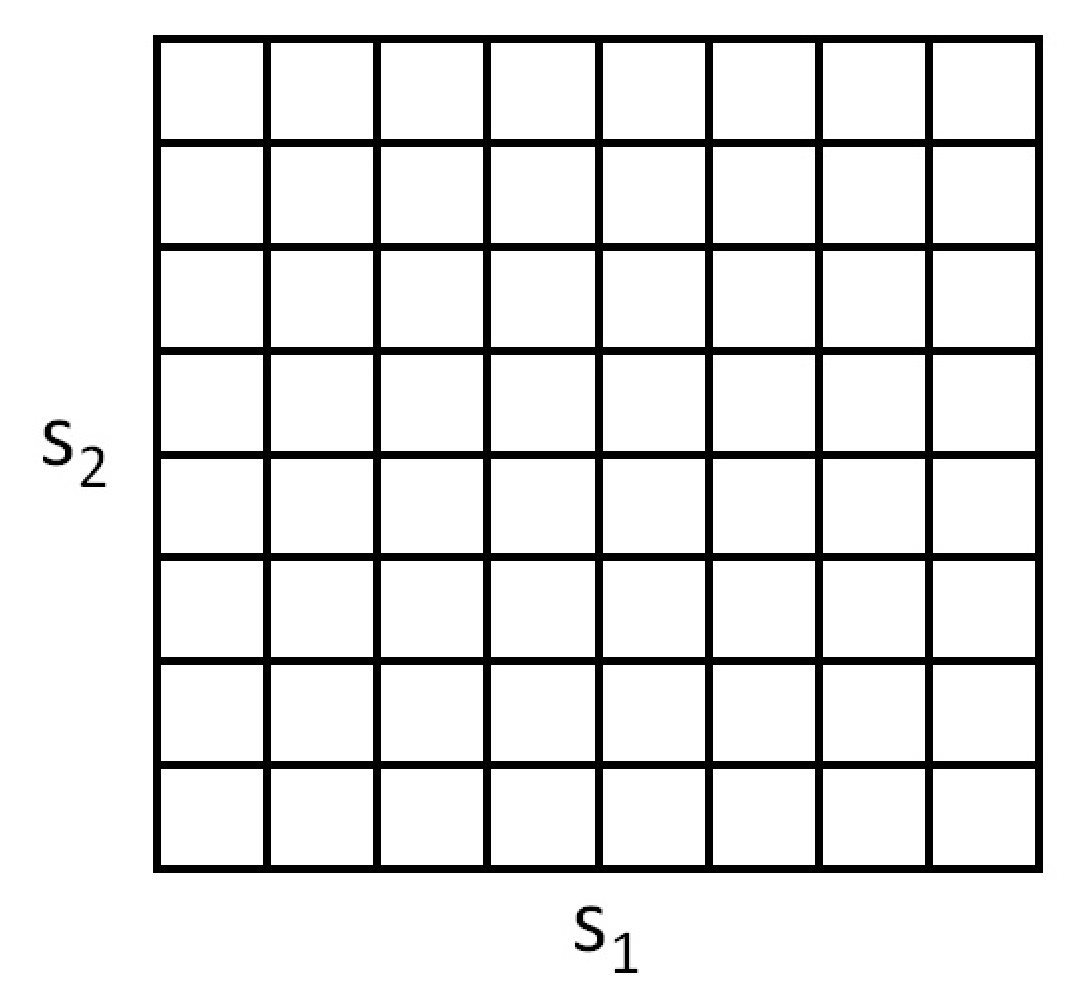
\includegraphics[scale=0.3]{gridDiscretization.eps}
\end{center}
Here, each grid cell represents a separate discrete state $\sbar$.
We can then approximate the continuous-state MDP via a discrete-state one
$(\Sbar, A, \{P_{\sbar a}\}, \gamma, R)$, where $\Sbar$ is the set of
discrete states,
$\{P_{\sbar a}\}$ are our state transition probabilities over the discrete
states, and so on.  We can then use value iteration or policy iteration
to solve for the $\Vstar(\sbar)$ and $\pistar(\sbar)$ in the discrete state
MDP
$(\Sbar, A, \{P_{\sbar a}\}, \gamma, R)$.  When our actual system is in
some continuous-valued state $s \in S$ and we need to pick an action to execute, we compute the corresponding
discretized state $\sbar$, and execute action $\pistar(\sbar)$.

This discretization approach can work well for many problems.  However, there are
two downsides.  First, it uses a fairly naive representation
for $\Vstar$ (and $\pistar$).  Specifically, it assumes that the value
function is takes a constant value over each of the discretization intervals
(i.e., that the value function is piecewise constant in each of the gridcells).

To better understand the limitations of such a representation, consider
a \emph{supervised learning} problem of fitting
a function to this dataset:
\begin{center}
% eps library outdated
% \epsfxsize=3in
% \epsffile{linearData.eps}
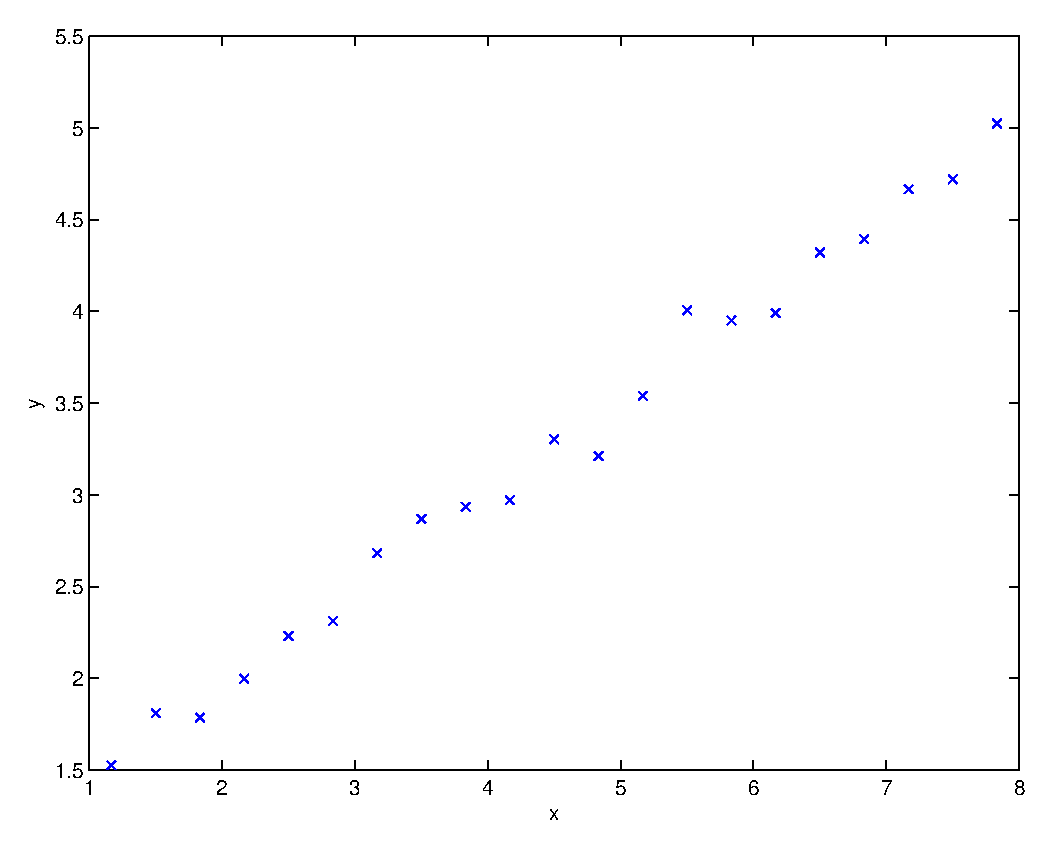
\includegraphics[scale=0.4]{linearData.eps}
\end{center}

Clearly, linear regression would do fine on this problem.  However, if we instead
discretize the $x$-axis, and then use a
representation that is piecewise constant in each
of the discretization intervals, then our fit to the data would look
like this:
\begin{center}
% eps library outdated
% \epsfxsize=3in
% \epsffile{staircase.eps}
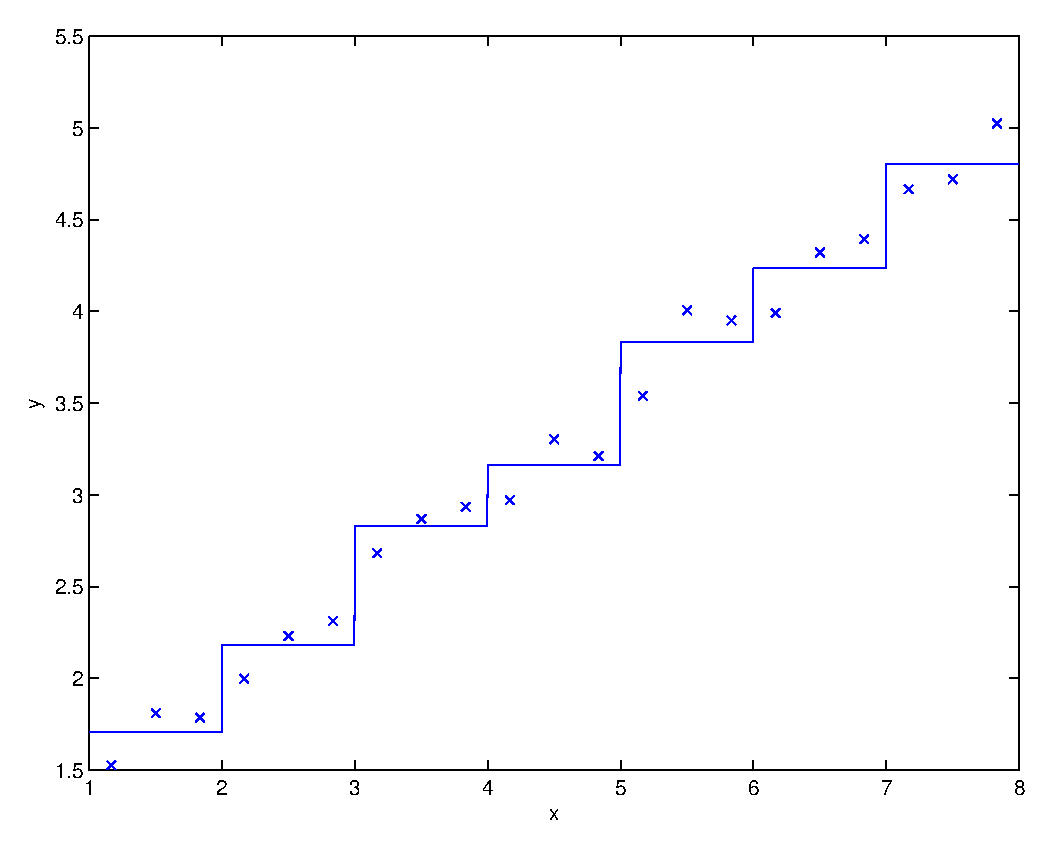
\includegraphics[scale=0.4]{staircase.eps}
\end{center}

This piecewise constant representation just isn't a good representation for
many smooth functions.  It results in little smoothing over the inputs, and no
generalization over the different grid cells.  Using this sort of representation,
we would also need a very fine discretization (very small grid cells) to get a good approximation.

A second downside of this representation is called the {\bf curse of
dimensionality}.  Suppose $S = \Re^\di$, and we discretize each of the $\di$
dimensions of the state
into $k$ values.  Then the total number of discrete states we have is
$k^\di$.  This grows exponentially quickly in the dimension of the state space $\di$,
and thus does not scale well to large problems.  For example, with a 10d state,
if we discretize each state variable into 100 values, we would have
$100^{10} = 10^{20}$ discrete states, which is far too many to represent even on
a modern desktop computer.

As a rule of thumb, discretization usually works extremely well for 1d and 2d
problems (and has the advantage of being simple and quick to implement).
Perhaps with a little bit of cleverness and some care in choosing the
discretization method, it often works well for problems with up to 4d states.  If
you're extremely clever, and somewhat lucky, you may even get it to work for
some 6d problems.  But it very rarely works for problems any higher
dimensional than that.


\subsection{Value function approximation} \label{sec-valuefunapprox}

We now describe an alternative method for finding policies in continuous-state MDPs, in
which we approximate $\Vstar$
directly, without resorting to discretization.  This approach, called value function
approximation, has been successfully applied to many RL problems.

\subsubsection{Using a model or simulator}

To develop a value function approximation algorithm, we will assume that we have a {\bf model}, or {\bf simulator}, for the MDP.
Informally, a simulator is a black-box that takes as input any (continuous-valued) state $s_t$ and action $a_t$,
and outputs a next-state $s_{t+1}$ sampled according to the state transition probabilities
$P_{s_ta_t}$:
\begin{center}
% eps library outdated
% \epsfxsize=3in
% \epsffile{simulator.eps}
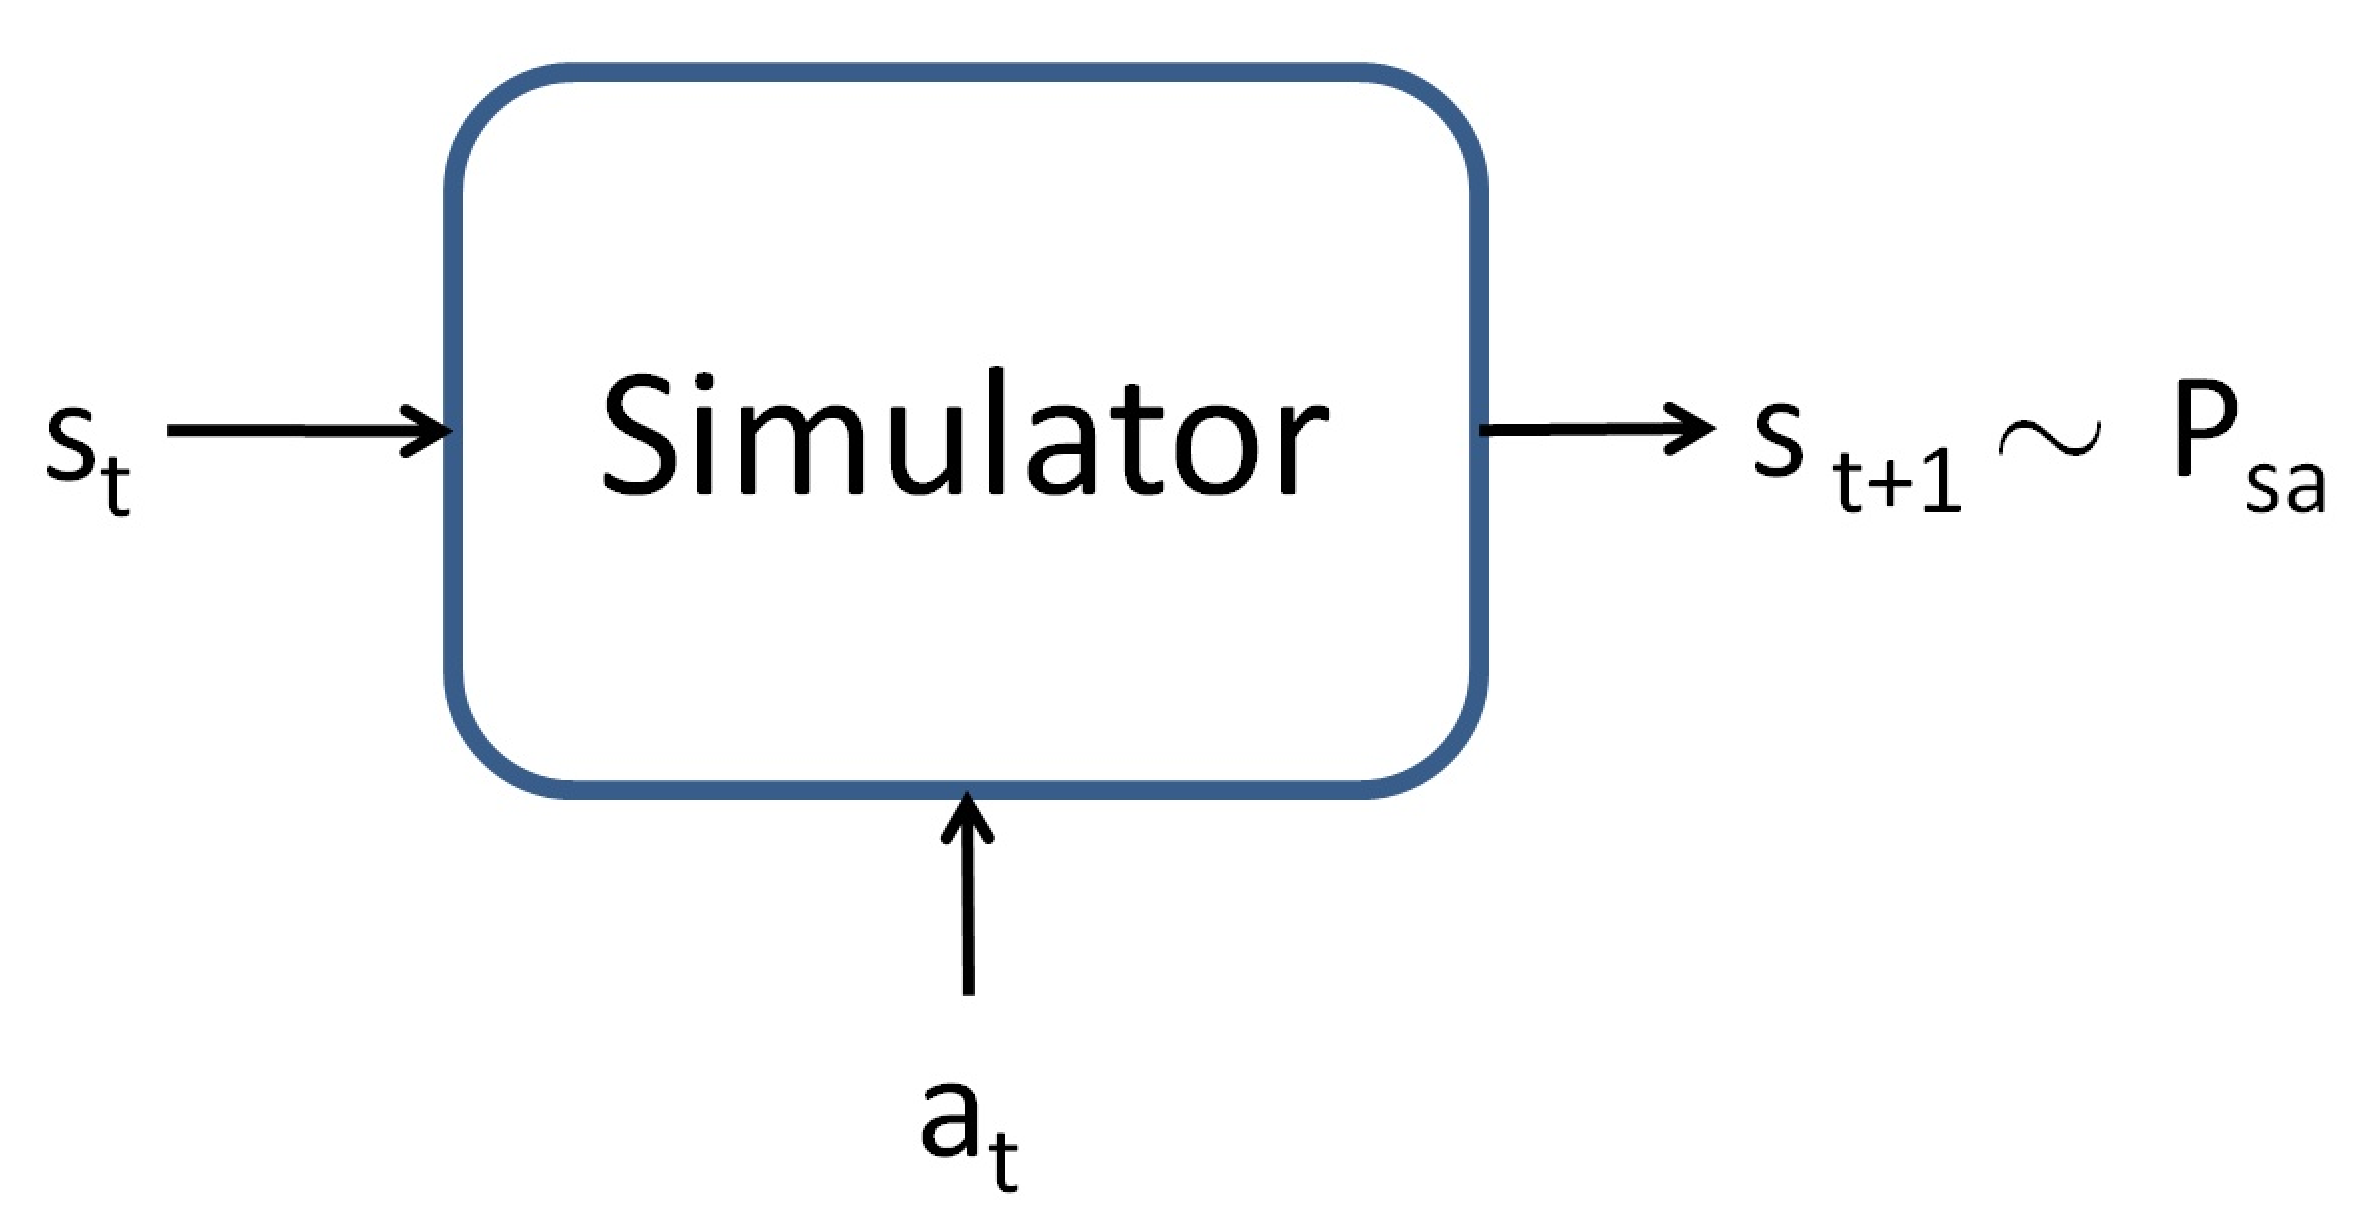
\includegraphics[scale=0.2]{simulator.eps}
\end{center}

There are several ways that one can get such a model.  One is to use physics
simulation.  For example, the simulator for the inverted pendulum in PS4 was
obtained by using the laws of physics to calculate what position and
orientation the cart/pole will be in at time $t+1$, given the current state at
time $t$ and the action $a$ taken, assuming that we know all the parameters of
the system such as the length of the pole, the mass of the pole, and so on.
Alternatively, one can also use an off-the-shelf physics simulation software
package which takes as input a complete physical description of a mechanical
system, the current state $s_t$ and action $a_t$, and computes the state
$s_{t+1}$ of the system a small fraction of a second into the
future.\footnote{Open Dynamics Engine (http://www.ode.com) is one example of
a free/open-source physics simulator that can be used to simulate systems like the
inverted pendulum, and that has been a reasonably popular choice among RL
researchers.}

An alternative way to get a model is to learn one from data collected in the MDP.  For example, suppose we
execute $\nexp$ {\bf trials} in which we repeatedly take actions in an MDP, each trial
for $T$ timesteps.  This can be done picking actions at random, executing some specific policy,
or via some other way of choosing actions.  We would then observe $\nexp$ state sequences like the following:
\begin{eqnarray*}
&s_0^{(1)} \stackrel{a_0^{(1)}}{\longrightarrow} s_1^{(1)} \stackrel{a_1^{(1)}}{\longrightarrow} s_2^{(1)}
\stackrel{a_2^{(1)}}{\longrightarrow} \cdots \stackrel{a_{T-1}^{(1)}}{\longrightarrow} s_T^{(1)} \\
&s_0^{(2)} \stackrel{a_0^{(2)}}{\longrightarrow} s_1^{(2)} \stackrel{a_1^{(2)}}{\longrightarrow} s_2^{(2)}
\stackrel{a_2^{(2)}}{\longrightarrow} \cdots \stackrel{a_{T-1}^{(2)}}{\longrightarrow} s_T^{(2)} \\
&\cdots \hbox to 2.1in{}\\
&s_0^{(\nexp)} \stackrel{a_0^{(\nexp)}}{\longrightarrow} s_1^{(\nexp)} \stackrel{a_1^{(\nexp)}}{\longrightarrow} s_2^{(\nexp)}
\stackrel{a_2^{(\nexp)}}{\longrightarrow} \cdots \stackrel{a_{T-1}^{(\nexp)}}{\longrightarrow} s_T^{(\nexp)}
\end{eqnarray*}
We can then apply a learning algorithm to predict $s_{t+1}$ as a function of $s_t$ and $a_t$.

For example, one may choose to learn a linear model of the form
\begin{equation}
s_{t+1} = A s_{t} + B a_{t},             \label{eqn-linearModel}
\end{equation}
using an algorithm similar to linear regression.  Here, the parameters of the model are
the matrices $A$ and $B$, and we can estimate them using the data collected from our $\nexp$ trials,
by picking
\begin{equation*}
\arg \min_{A,B} \sum_{i=1}^\nexp \sum_{t=0}^{T-1} \left\| s^{(i)}_{t+1} - \left(A s^{(i)}_t + B a^{(i)}_t\right) \right\|_2^2.
\end{equation*}
(This corresponds to the maximum likelihood estimate of the parameters.)

We could also potentially use other loss functions for learning the model. For example, it has been found in recent work~\cite{luo2018algorithmic} that using $\|\cdot\|_2$ norm (without the square) may be helpful in certain cases. 

Having learned $A$ and $B$, one option is to build a {\bf deterministic} model, in which given
an input $s_t$ and $a_t$, the output $s_{t+1}$ is exactly determined.  Specifically, we always
compute $s_{t+1}$ according to Equation~(\ref{eqn-linearModel}).
Alternatively, we may also build a {\bf stochastic} model, in which $s_{t+1}$ is a random function
of the inputs, by modeling it as
\[
s_{t+1} = A s_{t} + B a_{t} + \epsilon_t,
\]
where here $\epsilon_t$ is a noise term, usually modeled as $\epsilon_t \sim {\cal N}(0,\Sigma)$.
(The covariance matrix $\Sigma$ can also be estimated from data in a straightforward way.)

%In our discussion on LQR control, we'll later see that there're particularly effective algorithms
%for solving certain classes of linear MDPs, in which $s_{t+1}$ is a linear function of $s_{t}$ and
%$a_{t}$ (plus noise).

Here, we've written the next-state $s_{t+1}$ as a linear function of the current state
and action; but of course, non-linear functions are also possible.
Specifically, one can learn
a model $s_{t+1} = A \phi_s(s_{t}) + B \phi_a(a_{t})$, where
$\phi_s$ and $\phi_a$ are some non-linear feature mappings of the states and
actions.   Alternatively, one can also use non-linear learning algorithms, such as locally weighted linear
regression, to learn to estimate $s_{t+1}$ as a function of $s_t$ and $a_t$.
These approaches can also be used to build either deterministic or stochastic simulators
of an MDP.
%All of the algorithms described in Section~\ref{sec-valuefunapprox} will apply
%equally well to such non-linear models as well.

\subsubsection{Fitted value iteration}

We now describe the {\bf fitted value iteration} algorithm for approximating
the value function of a continuous state MDP.  In the sequel, we will assume
that the problem has a continuous state space $S = \Re^\di$, but that the action
space $A$ is small and discrete.\footnote{In practice, most MDPs have much
smaller action spaces than state spaces. E.g., a car has a 6d state space, and a
2d action space (steering and velocity controls); the inverted pendulum has a
4d state space, and a 1d action space; a helicopter has a 12d state space, and a
4d action space.  So, discretizing this set of actions is usually less of a
problem than discretizing the state space would have been.}

Recall that in value iteration, we would like to perform the update
\begin{eqnarray}
V(s) &:=& R(s) + \gamma \max_a \int_{s'} P_{sa}(s') V(s') ds' \\
&=& R(s) + \gamma \max_a \E_{s' \sim P_{sa}} [V(s')]        \label{eqn-viexpectation}
\end{eqnarray}
(In Section~\ref{sec-viandpi}, we had written the value iteration update
with a summation $V(s) := R(s) + \gamma \max_a \sum_{s'} P_{sa}(s') V(s')$
rather than an integral over states; the new notation reflects that we are now working
in continuous states rather than discrete states.)

The main idea of fitted value iteration
is that we are going to approximately carry out this step, over a finite sample
of states $s^{(1)}, \ldots, s^{(\nexp)}$.  Specifically, we will use a supervised learning
algorithm---linear regression in our description below---to approximate the value function
as a linear or non-linear function of the states:
\[
V(s) = \theta^T \phi(s).
\]
Here, $\phi$ is some appropriate
feature mapping of the states.

For each state $s$ in our finite sample of $\nexp$ states, fitted value iteration
will first compute a quantity $y^{(i)}$, which will be our approximation
to $R(s) + \gamma \max_a \E_{s' \sim P_{sa}} [V(s')]$ (the right hand side of
 Equation~\ref{eqn-viexpectation}).  Then, it will apply a supervised
learning algorithm to try to get $V(s)$ close to $R(s) + \gamma \max_a \E_{s' \sim P_{sa}} [V(s')]$
(or, in other words, to try to get $V(s)$ close to $y^{(i)}$).

In detail, the algorithm is as follows:

\begin{enumerate}
\item Randomly sample $\nexp$ states $s^{(1)}, s^{(2)}, \ldots s^{(\nexp)} \in S$.
\item Initialize $\theta := 0$.
\item Repeat $\{$
  \item[] \begin{enumerate}
    \item[] For $i=1,\ldots,\nexp$ $\{$
      \begin{enumerate}
      \item[] For each action $a \in A$ $\{$
      \item[] \begin{enumerate}
         \item[] Sample $s'_1, \ldots, s'_k \sim P_{s^{(i)}a}$ (using a model of the MDP).
         \item[] Set $q(a) = \frac{1}{k}\sum_{j=1}^k R(s^{(i)}) + \gamma V(s'_j)$
         \item[] $\;\;\;\;\;\; //$ Hence, $q(a)$ is an estimate of $R(s^{(i)}) + \gamma \E_{s' \sim P_{s^{(i)}a}}[V(s')]$.
      \end{enumerate}
      \item[] $\}$
      \item[] Set $y^{(i)} = \max_a q(a)$.
      \item[] $\;\;\;\;\;\; //$ Hence, $y^{(i)}$ is an estimate of $R(s^{(i)}) + \gamma \max_a \E_{s' \sim P_{s^{(i)}a}}[V(s')]$.
      \end{enumerate}
    \item[] $\}$
    \item[] $//$ In the original value iteration algorithm (over discrete states)
    \item[] $//$ we updated the value function according to $V(s^{(i)}) := y^{(i)}$.
    \item[] $//$ In this algorithm, we want $V(s^{(i)}) \approx y^{(i)}$, which we'll achieve
    \item[] $//$ using supervised learning (linear regression).
    \item[] Set $\theta := \arg \min_\theta \frac{1}{2} \sum_{i=1}^\nexp \left(\theta^T \phi(s^{(i)}) - y^{(i)}\right)^2$
  \end{enumerate}
  \item[] $\}$
\end{enumerate}

Above, we had written out fitted value iteration using linear regression as the algorithm to try to make
$V(s^{(i)})$ close to $y^{(i)}$.  That step of the algorithm is completely analogous to a standard
supervised learning (regression) problem in which we have a training set
$(x^{(1)}, y^{(1)}), (x^{(2)}, y^{(2)}), \ldots, (x^{(\nexp)}, y^{(\nexp)})$, and want to learn
a function mapping from $x$ to $y$; the only difference is that here $s$ plays the role of $x$.
Even
though our description above used linear regression, clearly other regression algorithms
(such as locally weighted linear regression) can also be used.

Unlike value iteration over a discrete set of states, fitted value iteration cannot be proved to always to converge.
However, in practice, it often does converge (or approximately converge), and works well for many problems.
Note also that if we are using a deterministic simulator/model of the MDP, then fitted value iteration can be
simplified by setting $k=1$ in the algorithm.
This is because the expectation in Equation~(\ref{eqn-viexpectation}) becomes an expectation over
a deterministic distribution, and so a single example is sufficient to exactly compute that expectation.
Otherwise, in the algorithm above, we had to draw $k$ samples, and average to try to approximate that
expectation (see the definition of $q(a)$, in the algorithm pseudo-code).

Finally, fitted value iteration outputs $V$, which is an approximation to $\Vstar$.  This implicitly defines
our policy.  Specifically,
when our system is in some state $s$, and we need to choose an action, we would like to choose the action
\begin{equation}
\arg \max_a \E_{s'\sim P_{sa}}[V(s')]                \label{eqn-pickaction}
\end{equation}
The process for computing/approximating this is similar to the inner-loop of fitted value iteration, where
for each action, we sample $s'_1, \ldots, s'_k \sim P_{sa}$ to approximate the expectation.  (And again,
if the simulator is deterministic, we can set $k=1$.)

In practice, there are often other ways to approximate this step as well.  For example, one very common
case is if the
simulator is of the form $s_{t+1} = f(s_t, a_t) + \epsilon_t$, where $f$ is some deterministic function
of the states (such as $f(s_t,a_t) = As_t+Ba_t$), and $\epsilon$ is zero-mean Gaussian noise.  In this case,
we can pick the action given by
\[
\arg \max_a V(f(s,a)).
\]
In other words, here we are just setting $\epsilon_t = 0$ (i.e., ignoring the noise in the simulator),
and setting $k=1$.  Equivalent, this can be derived from Equation~(\ref{eqn-pickaction}) using
the approximation
\begin{eqnarray}
\E_{s'}[V(s')] &\approx& V(\E_{s'}[s'])  \\
&=& V(f(s,a)),
\end{eqnarray}
where here the expectation is over the random $s' \sim P_{sa}$.
So long as the noise terms $\epsilon_t$ are small, this will usually
be a reasonable approximation.

However, for problems that don't lend themselves
to such approximations, having to sample $k|A|$ states using the model, in order
to approximate the expectation above, can be computationally expensive.
\bibliographystyle{plain}
\bibliography{bib}
\end{document}
